\documentclass[11pt,letterpaper]{report}

% --- Paquetes Requeridos ---
\usepackage[utf8]{inputenc}
\usepackage[T1]{fontenc}
\usepackage{lmodern}
\usepackage[letterpaper, margin=2.5cm]{geometry}
\usepackage{amsmath,amssymb}
\usepackage{xcolor}
\usepackage{graphicx}
\usepackage{booktabs}
\usepackage{tabularx}
\usepackage{multirow}
\usepackage{parskip}
\usepackage{microtype}
\usepackage{soul}
\usepackage[hidelinks]{hyperref}

% --- Configuración de Estilo ---
\renewcommand{\familydefault}{\sfdefault} % Fuente sans-serif limpia y moderna
\setcounter{secnumdepth}{3}                % Permitir numeración de secciones

% --- Macro para Fichas de Indicador ---
\newcommand{\fichaIndicador}[9]{
  \noindent
  \begin{tabularx}{\textwidth}{p{0.25\textwidth}XX}
  \toprule
  \textbf{#1} & \multicolumn{2}{c}{\textbf{FICHA DE INDICADOR}} \\
  \midrule
  \textbf{Nombre del indicador} & \textbf{Objetivo del indicador} & \textbf{Fórmula del indicador} \\
  #2 & #3 & #4 \\
  \midrule
  \textbf{Código del indicador} & \textbf{Responsable de gestión} & \textbf{Resp. de carga y reporte} \\
  #5 & #6 & #7 \\
  \midrule
  \textbf{Meta anualizada} & \textbf{Frecuencia de reporte} & \textbf{Fecha de actualización} \\
  #8 & #9 & 19/06/25 \\
  \bottomrule
  \end{tabularx}
  \vspace{1.5em}
}

% --- Datos del Documento ---
\title{\textbf{\large MANUAL DE PROCESOS ESTRATÉGICOS}\\[0.5em] \textbf{\Huge Gestión Financiera a Nivel Estratégico}}
\author{\textbf{LOGO COLOGISTIC}}
\date{}

\begin{document}

\maketitle

% --- Control de Versiones ---
\begin{center}
\textbf{\large CONTROL DE VERSIONES}
\end{center}
\begin{tabularx}{\textwidth}{p{0.25\textwidth}p{0.2\textwidth}p{0.2\textwidth}X}
\toprule
\textbf{Aprobado por Acuerdo de} & \textbf{Fecha de Aprobación} & \textbf{Fecha de Vigencia} & \textbf{Notas de la versión} \\
\midrule
- & - & - & \begin{itemize} \item Versión inicial \end{itemize} \\
\bottomrule
\end{tabularx}

\newpage

% --- Índice General ---
\tableofcontents

\newpage

% ==========================================
\chapter{Generalidades}
% ==========================================

\section{Objetivo}
Asegurar la liquidación mensual de rentas y servicios especiales, en dólares, garantizando el margen de utilidad entre el costo de alquiler pagado al dueño y el cobro al cliente corporativo.

\section{Alcance}
Este procedimiento aplica desde la recopilación manual de movimientos y guías de servicio operativo, pasando por la facturación, y finaliza con la entrega de estados financieros y de utilidad a la Gerencia General. Involucra a la Subgerencia, Jefatura de Operaciones/Analista de Inventarios y al Contador externo.

\section{Base Legal}
\begin{enumerate}
  \item \textbf{NIIF 16:} Establece los principios para el reconocimiento, medición y presentación de los arrendamientos.
  \item \textbf{NIIF 15:} Ingresos de Actividades Ordinarias Procedentes de Contratos con Clientes.
  \item \textbf{Ley N° 32201:} Ley que establece un régimen excepcional del Impuesto a la Renta.
\end{enumerate}

\section{Definiciones}
\begin{itemize}
  \item \textbf{Liquidación de Servicios:} Cálculo detallado de los movimientos logísticos (paletizado, reempaque) para su posterior facturación.
\end{itemize}

\newpage

% ==========================================
\chapter{Disposiciones Complementarias}
% ==========================================

\section{Diagrama General de Procesos}

\begin{figure}[h!]
  \centering
  
\includegraphics[width=0.95\textwidth]{./images/media/image1.png}
  \caption{Extracto de la Matriz de Procesos Estratégicos}
\end{figure}

\begin{center}
  \small
  \begin{tabularx}{\textwidth}{p{0.15\textwidth}p{0.18\textwidth}XXp{0.25\textwidth}}
  \toprule
  \multicolumn{2}{c}{\textbf{Macro Proceso}} & \multicolumn{2}{c}{\textbf{Proceso}} & \multirow{2}{*}{\textbf{Procedimientos}} \\
  \cmidrule(r){1-2} \cmidrule(l){3-4}
  \textbf{Título} & \textbf{Líder} & \textbf{Título} & \textbf{Líder} & \\
  \midrule
  \multirow{3}{=}{Gestión Financiera} & \multirow{3}{=}{Subgerente / Contador} & Consolidación de Liquidaciones & Subgerente & 
  \begin{itemize} \item Liquidación de Servicios Logísticos \item Liquidación de Arrendamiento Fijo \end{itemize} \\
  \cmidrule{3-5}
  & & Gestión de Emisión Documental & Subgerente / Contador & 
  \begin{itemize} \item Emisión Manual de Factura Electrónica \item Validación y Envío de Comprobantes \end{itemize} \\
  \cmidrule{3-5}
  & & Control Financiero y Análisis & Subgerente / Contador & 
  \begin{itemize} \item Monitoreo de Margen Operativo y Utilidad \item Conciliación Bancaria y Gestión de Divisas \end{itemize} \\
  \bottomrule
  \end{tabularx}
\end{center}

\newpage

% ==========================================
\chapter{Procedimientos}
% ==========================================

% ------------------------------------------
\section{Liquidación de Servicios Logísticos}
% ------------------------------------------
\textbf{Líder:} Subgerente (Karla Pettrozi)

\textbf{Participantes:}
\begin{itemize}
  \item Analista de Inventarios
  \item Subgerente
  \item Cliente
\end{itemize}

\textbf{Descripción del Procedimiento:} \\
El procedimiento extrae los movimientos del Excel, calcula cargos adicionales y prorratea los días de almacenaje. Con esos datos el analista genera un borrador de liquidación en USD, que el subgerente revisa y envía al cliente. El cliente aprueba o rechaza el reporte; si lo rechaza, el proceso vuelve a iniciar. Con la aprobación final, el subgerente emite el visto bueno y el proceso concluye.

\begin{figure}[h!]
  \centering
  
\includegraphics[width=0.9\textwidth]{./images/media/image2.png}
  \vspace{0.5em}
  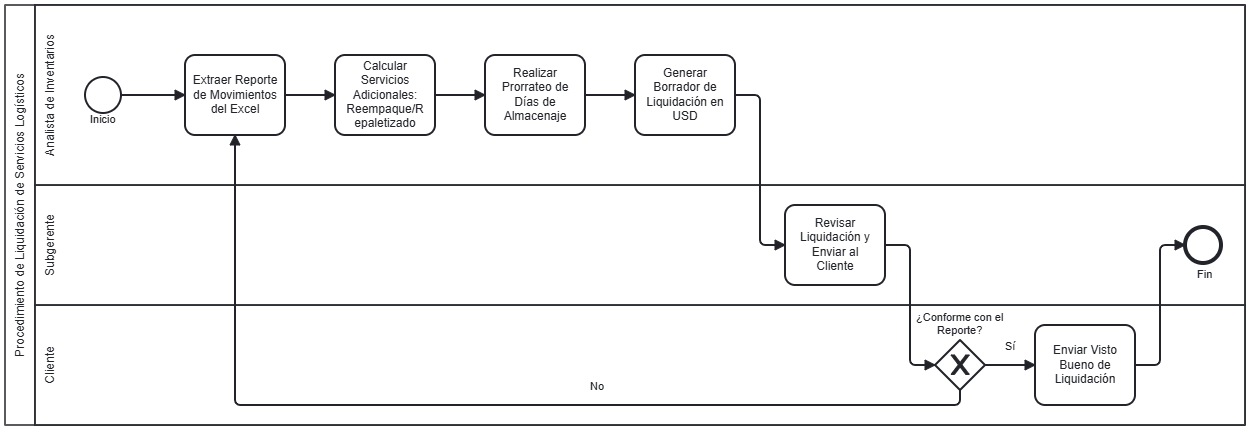
\includegraphics[width=0.9\textwidth]{./images/media/image3.png}
  \caption{Diagrama de Actividades con BPMN - Liquidación de Servicios Logísticos}
\end{figure}

\newpage

% ------------------------------------------
\section{Liquidación de Arrendamiento Fijo}
% ------------------------------------------
\textbf{Líder:} Subgerente

\textbf{Participantes:}
\begin{itemize}
  \item Subgerente
\end{itemize}

\textbf{Descripción del Procedimiento:} \\
El subgerente identifica los metros cuadrados ocupados según el contrato, multiplica esa área por la tarifa pactada para calcular la renta y genera el consolidado mensual de rentas, finalizando el proceso.

\begin{figure}[h!]
  \centering
  
\includegraphics[width=0.9\textwidth]{./images/media/image2.png}
  \vspace{0.5em}
  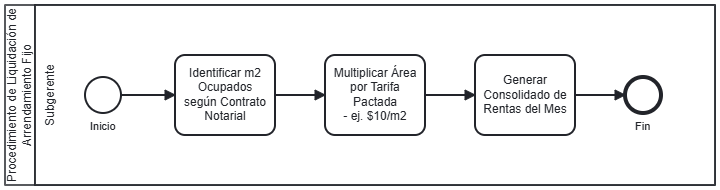
\includegraphics[width=0.9\textwidth]{./images/media/image4.png}
  \caption{Diagrama de Actividades con BPMN - Liquidación de Arrendamiento Fijo}
\end{figure}

\newpage

% ------------------------------------------
\section{Emisión Manual de Factura Electrónica}
% ------------------------------------------
\textbf{Líder:} Subgerente (Karla Pettrozi)

\textbf{Participantes:}
\begin{itemize}
  \item Gerencia General
  \item Contador
\end{itemize}

\textbf{Descripción del Procedimiento:} \\
Formalizar la generación, validación y envío de la factura electrónica a SUNAT de forma manual, asegurando la trazabilidad y el control de los pasos críticos por parte del Subgerente y el Contador.

\begin{figure}[h!]
  \centering
  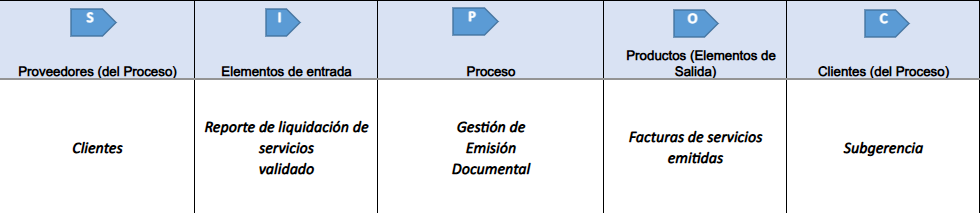
\includegraphics[width=0.9\textwidth]{./images/media/image5.png}
  \vspace{0.5em}
  
\includegraphics[width=0.9\textwidth]{./images/media/image6.png}
  \caption{Diagrama de Actividades con BPMN - Emisión Manual de Factura}
\end{figure}

\newpage

% ------------------------------------------
\section{Procedimiento de Validación y Envío de Comprobante}
% ------------------------------------------
\textbf{Líder:} Subgerente (Karla Pettrozi)

\textbf{Participantes:}
\begin{itemize}
  \item Gerencia General
\end{itemize}

\textbf{Descripción del Procedimiento:} \\
Se cruzan los ingresos facturados contra los costos fijos (alquiler base a los dueños) para determinar la rentabilidad. Se genera el informe final para la toma de decisiones estratégicas.

\begin{figure}[h!]
  \centering
  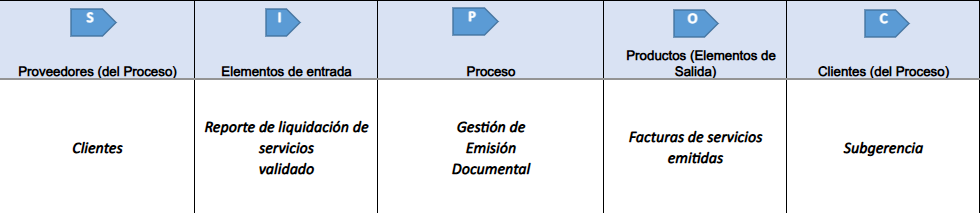
\includegraphics[width=0.9\textwidth]{./images/media/image5.png}
  \vspace{0.5em}
  
\includegraphics[width=0.9\textwidth]{./images/media/image7.png}
  \caption{Diagrama de Actividades con BPMN - Validación y Envío}
\end{figure}

\newpage

% ------------------------------------------
\section{Procedimiento de Monitoreo de Margen Operativo y Utilidad}
% ------------------------------------------
\textbf{Líder:} Subgerente (Karla Pettrozi)

\textbf{Participantes:}
\begin{itemize}
  \item Gerencia General
  \item Contador
\end{itemize}

\textbf{Descripción del Procedimiento:} \\
Se cruzan los ingresos facturados contra los costos fijos (alquiler base a los dueños) para determinar la rentabilidad. Se genera el informe final para la toma de decisiones estratégicas.

\begin{figure}[h!]
  \centering
  
\includegraphics[width=0.9\textwidth]{./images/media/image8.png}
  \vspace{0.5em}
  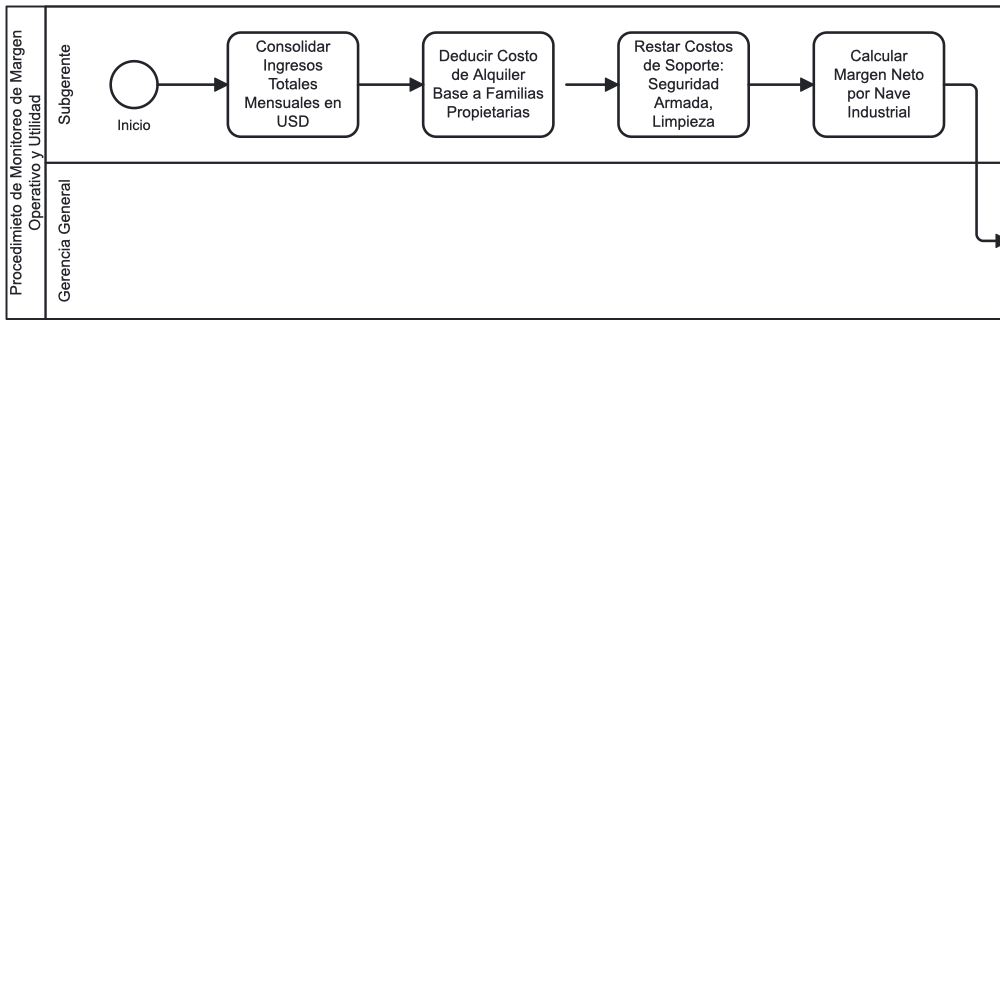
\includegraphics[width=0.9\textwidth]{./images/media/image10}
  \caption{Diagrama de Actividades con BPMN - Monitoreo de Margen}
\end{figure}

\newpage

% ------------------------------------------
\section{Procedimiento de Conciliación Bancaria y Gestión de Divisas}
% ------------------------------------------
\textbf{Líder:} Subgerente (Karla Pettrozi)

\textbf{Participantes:}
\begin{itemize}
  \item Gerencia General
  \item Contador
\end{itemize}

\textbf{Descripción del Procedimiento:} \\
Se cruzan los ingresos facturados contra los costos fijos (alquiler base a los dueños) para determinar la rentabilidad. Se genera el informe final para la toma de decisiones estratégicas.

\begin{figure}[h!]
  \centering
  
\includegraphics[width=0.9\textwidth]{./images/media/image8.png}
  \vspace{0.5em}
  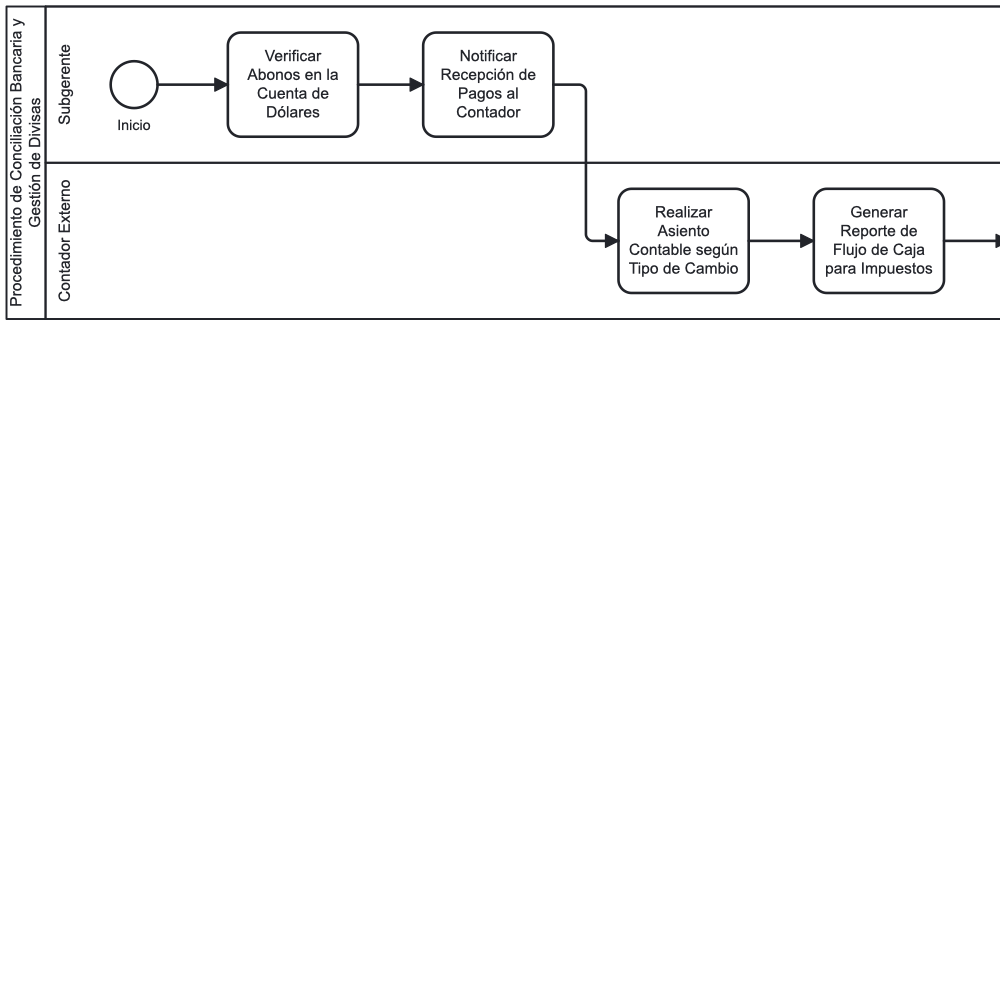
\includegraphics[width=0.9\textwidth]{./images/media/image12}
  \caption{Diagrama de Actividades con BPMN - Conciliación y Divisas}
\end{figure}

\newpage

% ==========================================
\chapter{Matriz de Indicadores}
% ==========================================

\fichaIndicador{1. Mezclado}{Precisión en el mezclado}{Medir el porcentaje de mezclas realizadas con cantidades exactas de ingredientes según receta}{(Nº de mezclas correctas / Nº total de mezclas realizadas) $\times$ 100}{AP-001}{Jefe de Producción}{Supervisor de Mezclado}{98\%}{Mensual}

\fichaIndicador{2. Amasado y pesado}{Precisión en el peso de masa}{Controlar que el peso de las porciones de masa esté dentro del margen permitido}{(Nº de porciones con peso correcto / Nº total de porciones verificadas) $\times$ 100}{AP-002}{Jefe de producción}{Supervisor de Amasado y Pesado}{90\%}{Mensual}

\fichaIndicador{3. Formado}{Tiempo promedio de autorización}{Medir el porcentaje de piezas formadas que cumplen con los estándares de tamaño y forma}{(Nº de piezas correctas / Nº total de piezas formadas) $\times$ 100}{AP-003}{Jefe de Producción}{Supervisor del área de formado}{100\%}{Mensual}

\fichaIndicador{4. Limpieza del molde}{Eficiencia en limpieza y engrasado}{Verificar el cumplimiento del protocolo de limpieza y engrasado antes del uso del molde}{(Nº de moldes correctamente engrasados y limpios / Nº total de moldes utilizados) $\times$ 100}{AP-004}{Supervisor de Calidad}{Encargado de limpieza y preparación de moldes}{100\%}{Mensual}

\fichaIndicador{5. Bañado}{Cobertura uniforme}{Medir el porcentaje de productos bañados correctamente según los estándares de calidad}{(Nº de productos con bañado uniforme / Nº total de productos bañados) $\times$ 100}{AP-005}{Supervisor de Producción}{Supervisor de Producción}{100\%}{Mensual}

\fichaIndicador{6. Fermentado}{Control de fermentación}{Medir el porcentaje de productos que cumplen con el tiempo y condiciones óptimas de levado}{(Nº de productos bien fermentados / Nº total de productos fermentados) $\times$ 100}{AP-006}{Jefe de Producción}{Encargado del fermentado}{100\%}{Mensual}

\fichaIndicador{7. Horneado}{Producto horneado óptimo}{Evaluar el porcentaje de productos horneados con el punto exacto de cocción y sin defectos}{(Nº de productos correctamente horneados / Nº total de productos horneados) $\times$ 100}{AP-007}{Jefe de Producción}{Encargado del horno}{100\%}{Mensual}

\fichaIndicador{8. Enfriado}{Tiempo de enfriado}{Medir el tiempo promedio en que los productos alcanzan la temperatura óptima para su almacenamiento y consumo.}{(Nº de productos enfriados en el tiempo objetivo / Nº total de productos enfriados) $\times$ 100}{AP-008}{Jefe de Producción}{Supervisor de Enfriado}{100\%}{Mensual}

\fichaIndicador{9. Corte}{Precisión en el corte}{Medir el porcentaje de cortes realizados con precisión según las medidas establecidas en la orden de producción.}{(Nº de cortes precisos / Nº total de cortes realizados) $\times$ 100}{AP-002}{Jefe de Producción}{Encargado de Corte}{100\%}{Mensual}

\fichaIndicador{10. Empaquetado}{Eficiencia en el empaquetado}{Medir el porcentaje de productos empaquetados correctamente y de acuerdo con los estándares establecidos.}{(Nº de productos empaquetados correctamente / Nº total de productos empaquetados) $\times$ 100}{AP-010}{Jefe de Producción}{Supervisor de Empaque}{100\%}{Mensual}

\fichaIndicador{11. Etiquetado}{Etiquetado de productos terminados}{Medir el porcentaje de productos etiquetados correctamente, con información legible y conforme a los estándares de presentación establecidos.}{(N° de productos etiquetados correctamente / N° total de productos etiquetados) $\times$ 100}{AP-004}{Jefe de Producción}{Encargado de etiquetado}{100\%}{Mensual}

\newpage

% ==========================================
\chapter{Documentos Generados}
% ==========================================

\begin{tabularx}{\textwidth}{XXXX}
\toprule
\multirow{2}{*}{\textbf{DOCUMENTO (QUÉ)}} & \multicolumn{3}{c}{\textbf{CUSTODIA}} \\
\cmidrule{2-4}
& \textbf{QUIÉN} & \textbf{DÓNDE} & \textbf{CÓMO} \\
\midrule
- & - & - & - \\
- & - & - & - \\
\bottomrule
\end{tabularx}

\vspace{3em}

% ==========================================
\chapter{Anexos}
% ==========================================
\textbf{ANEXO N° 01:} [Título del Anexo] \\
\textbf{ANEXO N° 02:} [Título del Anexo]

\end{document}
